\chapter{Artificial Neural Networks}
Artificial neural networks are a specific flavor of machine learning that are loosely inspired by neural operation in the human brain and are able to classify or regress data, or to serve as a controller.

While artificial neural networks have long time been one out of many go-to methods from the vast field of machine learning to address these problems, recent advances in computing, in particular graphical processing units (GPU) and the availability of large datasets, which in turn resulted into the ability to train very, very large neural networks, also known as ``deep learning'', that have led to revolutionary results in many fields including computer vision, natural language processing, video and speech processing, and robotics.

Not too long ago, neural networks have been considered ``deep'' with more than two layers. Today, ``deep'' neural networks can have hundreds of layers and thousands of inputs and output, or more. This is still shy of the human brain, or even tiny areas thereof, which contains 100 billion neurons, each with thousands of synapses connecting a single neuron to thousands of others.

\section{When to use machine learning?}
Machine learning is a large field that shares many of the foundations in probability theory and statistics with robotics. The goal of this chapter is to provide a basic understanding of simple and recurrent neural networks that is sufficient to connect these tools to other topics in this book. In particular, deep learning can be used as a drop-in replacement for forward and inverse kinematics, sensor preprocessing and conditioning, computer vision and feature extraction, localization, and even replace controllers for locomotion and grasping. Here, it is important to understand when deep learning models might provide better solutions as well as when they do not. In a nutshell, deep learning models become first choice when not enough information exist to model a system using first principles. While a ``deep enough'' model with the right architecture might approximate any existing function in robotics, deep learning models lack ``explainability'' beyond statistical accuracy, that is, we do not know why the approach actually works and when it might fail, usually making it second choice over an approach based on first principles.  


\section{The simple Perceptron}
Artificial neural networks are inspired by neurons and synapses in the human brain and have been studied since the 1950ies. One of the earliest model is the \index{Perceptron}\index{Simple Perceptron}\emph{Perceptron}, which can classify an input vector $x$ of dimension $m$ into two classes. Such a problem is shown in Figure \ref{fig:linearsep}. Variations of the simple perceptron remain the basic elements of deep neural networks till today.

\begin{figure}[!htb]
\centering
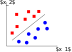
\includegraphics[width=0.5\columnwidth]{figs/linearlyseparable}
\caption{A 2-dimensional dataset (every element has two values $x_1$ and $x_2$) consisting of two classes, red and blue, that can be separated by a straight line.\label{fig:linearsep}}
\end{figure}

Formally, a Perceptron has $m$ inputs, $x_1$ to $x_m$, each modulated by a weight $w_1$ to $w_m$, respectively, as well as a treshold $b$, and outputs either zero or one (Figure \ref{fig:perceptron}). This is schematically illustrated in Figure \ref{fig:perceptron}.

\begin{figure}[!htb]
\centering
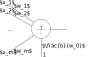
\includegraphics[width=0.5\columnwidth]{figs/perceptron.png}
\caption{The simple perceptron passes the dot product between the inputs $x$ and weights $w$ through a Heaviside function, returning 1 when $wx+b>0$ and 0 otherwise\label{fig:perceptron}}.
\end{figure}

The Perceptron classifies whether $x$ lies above or below a hyperplane defined by the weights $w$ using the following equation:
%
\begin{equation}
f(x)=\begin{cases}
1 \qquad wx+b > 0\\
0 \qquad otherwise
\end{cases}
\end{equation}
%
Here, $wx=\sum_{i=1}^mw_ix_i$ is the dot product and the non-linear activation function is also known as \index{Heaviside step function}\emph{Heaviside step function}. In practice, we are appending the value of '1' to the vector $x$ so that $x_0=1$, which simplifies $wx+b$ to $wx$ where $w_0$ taking up the role of $b$. This is illustrated in Figure \ref{fig:perceptron}, where the bias $b$ is alternatively labeled by $w_0$ and input $x_0=1$.


\subsection{Geometric interpretation of the simple perceptron}
If $w$ really defines a hyperplane, we should be able to see it when $m=2$. When $m=2$, that is every data point $x$ has only 2 dimensions, the separating hyperplane is a line. This can be seen as follows: writing the dot product out yields
\begin{equation}
w_1x_1+w_2x_2+b=0
\end{equation}
As we plot $x_1$ along the x-axis and $x_2$ along the y-axis, we can write
\begin{equation}
w_1x+w_2y+b=0
\end{equation}
This can be rewritten into
\begin{equation}
y=-\frac{w1}{w2}x-\frac{b}{w_2}
\end{equation}
and displayed within a scatter plot.

\subsection{Training the simple Perceptron}
Training the Perceptron, that is finding appropriate values for $w$ and $b$ that separate the data into two classes, is a simple iterative process:

\begin{enumerate}
\item Initialize the weights with zeros or a small random number
\item Compute the prediction $y_j=f(wx_j+b)$ for each data point $x_j$. A suitable choice for $f()$ is the Heaviside step function, e.g.
\item Calculate the mismatch between prediction $y_j$ and the true class $d_j$ to update the weights
\begin{equation}
w(t+1)=w(t)+r(d_j-y_j)*x_j
\end{equation}
\end{enumerate}

Repeat steps 2 and 3 until a termination criteria, such as a decreasing error or maximum number of iterations, is reached.

Albeit very simple, this simple learning algorithm has still a lot in common with state-of-the-art algorithms. First, weights are updated in an iterative process using small increments governed by a parameter $r$, standing for \index{Learning Rate}\emph{learning rate}. By changing $w$ in small increments, the algorithm is literally rotating and translating the separating line in a direction that minimizes the \emph{loss}, given by $d_i-y_i$. One can easily see that if the learning rate is too low, the algorithm will never find a good solution. One can also see that if the learning rate is too large, the line might move too much, skipping the optimal pose.

Notice that this simple implementation is de facto implementing gradient descent on a loss function of the form $(d_i-y_i)^2$, that can be minimized by moving against the direction of its gradient, here $2(d_i-y_i)$.

Second, the learning algorithm requires multiple presentations of the data-set, as the error is computed for every point in the data set. The more data, the longer training takes, in this case the increase in time is linear, which is a good approximation also for modern learning algorithms.

Third, the error between prediction and true class is only calculated based on training data. Even if we train with unlimited amounts of data points, it is still difficult to answer how the algorithm generalizes for new data, and whether also these new measurements will be distributed as the training data.

\section{Activation Functions}
Using a on-off Heaviside step function makes training a neural network using gradient descent rather difficult as a function that switches from ``not working at all'' to ``working completely'' provides very little information in which direction to move. It is therefore more desirable to have a smooth activation function. One such function is the \index{Sigmoid function}\emph{sigmoid function}:
\begin{equation}
\sigma(x)=\frac{1}{1+e^{-x}}
\end{equation}
Its main characteristics are that it assymptotically stays between 0 and 1, and crosses the y-axis at 0.5. It is shown in Figure \ref{fig:activationfunctions}, left.

\begin{figure}[!htb]
\centering
\includegraphics[width=0.9\columnwidth]{figs/activationfunctions}
\caption{Typical activation functions used in neural networks, the Sigmoid activation function, left, and the rectified linear unit (ReLU).\label{fig:activationfunctions}}
\end{figure}

The sigmoid function is very attractive for learning as the direction in which the weights should move to improve the error is very clear in the vicinity of $wx=0$, and computing its derivative is rather simple as we see below. In case of $wx$ being very large, or very small, the neuron either saturates or never activates, also known as the \emph{vanishing gradient}problem. Another drawback is that computing the sigmoid function is computationally expensive. A similar function is the hyperbolic tangent $\tanh()$ which remains in the range of -1 to 1 and crosses the y-axis at 0.

A popular solution to decrease computation time is the \index{Rectified Linear Unit (ReLU)}\emph{Rectified Linear Unit} (ReLU), which is given by
\begin{equation}
R(x)=max(0,x)
\end{equation}
and is shown in Figure \ref{fig:activationfunctions}, right.The dashed line indicates a refinement of the ReLU known as \emph{leaky ReLU} with a slope of typical 0.1, and improves learning for negative $wx$ by providing a directional gradient.

Note that we only talk about ``Perceptrons'' when the Heaviside step function is used as activation function.

\section{From the simple Perceptron to Multi-layer neural networks}

We have seen that the single Perceptron is able to linearly separate a dataset, spitting out ``0'' or ``1'' as a function of the data being below or above the separating hyperplane defined by the weight vector $w$. It is easy to see that some problems cannot be linearly separated. This is illustrated in Figure \ref{fig:xorproblem}.

\begin{figure}[!htb]
\centering
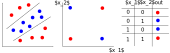
\includegraphics[width=0.9\columnwidth]{figs/xorproblem}
\caption{Data that cannot be separated using a single line (left) in canonical form (center). This problem is known as the ``XOR'' problem due to the truth table of the associated classification problem (right).\label{fig:xorproblem}}
\end{figure}

In the example above, the red and the blue data points are not separable by a single line, but require at least two lines. This problem is known as the ``XOR'' problem, which can be seen by looking at just four data points at $(0,0)$, $(0,1)$, $(1,0)$, and $(1,1)$. Tabulating this data togethwer with its color, reveals a truth table with the characteristics of logical exclusive or (XOR), that is $x_1$ and $x_2$ have to be different for the output to be true (here ``blue''), whereas the output is false (here ``red'') when the inputs are the same.

We already know that a single Perceptron can create a single separating hyperplane, we will therefore need at least two Perceptrons to solve the XOR problem. Using two Perceptrons in parallel will yield us with tuples of the kind $(0,0)$, $(0,1)$ and so on. We therefore need one more Perceptron to recombine these tuples into a single output. Figure \ref{fig:basicmultilayer}
shows the simple-most multi-layer Perceptron that can be trained for the XOR problem, with one \index{Input Layer}\emph{input layer}, a so-called\index{Hidden Layer} \emph{hidden layer}, and an \index{Output Layer}\emph{output layer}.

\begin{figure}
\centering
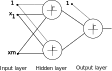
\includegraphics[width=0.8\columnwidth]{figs/basicmultilayernetwork}
\caption{A simple multi-layer perceptron with one input, one hidden, and one output layer. \label{fig:basicmultilayer}}
\end{figure}

\subsection{Formal description of Artificial Neural Networks}
As with the simple Perceptron, we will use node i's bias as the 0-th weight vector, that is
\begin{equation}
w^k_{0,j}=b^k_j
\end{equation}
Here, we use the following notation. We will denote the layer with a superscript, and the index of the incoming node and the outgoing node with a subscript tuple. That is $w^k_{i,j}$ is connecting the i-th incoming weight to the $j-th$ node of the $k-th$ layer. (The i-th incoming weight is the j-th node in layer $k-1$.) This, as well as the simple example network from above, are illustrated in Figure \ref{fig:backpropnotation}.

\begin{figure}[!htb]
\centering
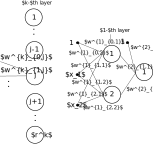
\includegraphics[width=0.7\columnwidth]{figs/backpropnotation}
\caption{Notation used to index weights (left) with respect to layer $k$ and the multi-layer network from Figure \ref{fig:basicmultilayer} (right).\label{fig:backpropnotation}}
\end{figure}

Each layer, denoted by the index $k$, has exactly $r^k$ nodes.

\subsection{Inputs and outputs}

The output $o_i$ of output node $i$ is given by
\begin{equation}
o_i=g(a_i^k)
\end{equation}
where $g()$ is a non-linear activation function such as --- but not limited to --- the Heaviside step function. Here, $a_i^k$ is the weighted sum computed by node $i$ in layer $k$, also known as the \index{Activation (neural network)}\emph{activation}:
\begin{equation}
a_i^k=\sum_{j=0}^{r_{k-1}}w_{j,i}^ko_j^{k-1}
\end{equation}
with $o_j^{k-1}$ the j-th output of the previous layer. This is illustrated in Figure \ref{fig:backpropnotation2}.

\begin{figure}[!htb]
\centering
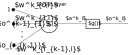
\includegraphics[width=0.7\columnwidth]{figs/backpropnotation2}
\caption{Inputs and outputs of neuron $i$ in the $k$-th layer showing activation $a_i$ and output $o_i$.\label{fig:backpropnotation2}}
\end{figure}

In case of $k$ being the output layer, $o_i^k$ should be equivalent to $y_i^k$. Likewise, in case of $k-1$ being the input layer $o_i^{k-1}=x_i$.

\subsection{Training a multi-layer neural network}

Finding a set of weights and bias values, that is 9 parameters for a simple two-dimensional problem, but potentially millions for a ``deep network'', is an NP-complete problem \cite{blum1992training}. We therefore need a smart approximative algorithm. We consider a training dataset consisting of input-output pairs $x_i$ and ouput $y_i$ with $i=1..N$, and a feedforward neural network with parameters $w$.

\subsubsection{Loss function}
The goal of training is to minimize an error function such as the mean squared error
\begin{equation}
E(x,y,w)=\frac{1}{2N}\sum_{i=1}^{N}(\hat{y_i}-y_i)^2
\end{equation}
between the output $\hat{y_i}$ that the neural network with parameters $w$ computes and the known value $y_i$ from what is known as the \index{Training set}\emph{training set}.

Similar to the Perceptron, we can reduce $E(x,y,w)$ by iteratively descending along its gradient, that is
\begin{equation}
w(t+1)=w(t)-\alpha \frac{\partial E(x,y,w(t))}{\partial w}
\end{equation}

\subsubsection{Backpropagation}
Calculating the partial derivatives for the error function manually is not straightforward as the neural network implements a computation graph, transforming the input $x$ by a series of multiplications and non-linear activation functions, which in turn require the chain rule.

Applying the chain rule can be done in two ways: moving forwards or backwards through the computation graph. Actually doing this by hand for a simple graph shows that going backwards is significantly more efficient. Manually deriving the individual partial derivatives also illustrates that many of the computations can actually be recycled. This solution is known as \index{Backpropagation}\emph{backpropagation} \cite{rumelhart1985learning}, a technique that has been independently discovered in multiple fields. The derivation below follows \cite{backpropagation}.

In a first step, we note that the error function is a sum over all input-output pairs:
\begin{equation}
\frac{\partial E(x,y,w)}{\partial w_{i,j}^k}=\frac{1}{2N}\sum^N_{d=1}\frac{\partial}{\partial w_{i,j}^k}(\hat{y_d}-y_d)^2=\frac{1}{2N}\sum_{d=1}^N\frac{\partial E_d}{\partial w_{i,j}^k}
\end{equation}
We will therefore focus on only one input-output pair $(x_d,y_d)$ and differentiate against $w_{i,j}^k$. (The index $d$ has been chosen to avoid confusion with the indices $i$ and $j$, and will be omitted for brevity in the remainder).

\paragraph{The Chain rule} The key for understanding the backpropagation algorithm is to apply the chain rule in a correct way. Specifically, if a variable $z$ depends on the variable $y$, which itself depends on the variable $x$, then
\begin{equation}
\frac{dz}{dx}=\frac{dz}{dy}\frac{dy}{dx}
\end{equation}

With the output layer having index $m$ and a single output ($a^m_1$), the error is computed by the recursive formula
\begin{equation}
E(x,y,w_{i,j})=\frac{1}{2}(\hat{y}-y)^2=\frac{1}{2}(g(a_1^m)-y)^2=
\frac{1}{2}\left(g\left(\sum_{l=0}^{r_{m-1}}w_{l,1}^mo_l^{m-1}\right)-y\right)^2.
\end{equation}
We observe that the variable $E$ depends on the outputs $o_l^{m-1}$ with $l=0..r_{m-1}$ from the previous layer. Recall that $o_l^{m-1}$ is simply the activation $a_l^{m-1}$ after applying the activation function. Also recall that $w^m_{i,1}$ are weights coming into node $1$. The error with respect to $w_{i,j}$ is therefore dependent on all $a^k_j$ for all previous layers. This is also visualized in Figure \ref{fig:backpropnotation3}.

\begin{figure}[!htb]
\centering
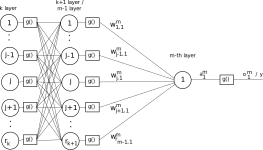
\includegraphics[width=0.8\columnwidth]{figs/backpropnotation3}
\caption{Last three layers of a neural network with a single output neuron, illustrating dependencies between function values and the output when moving along the computation graph backwards.\label{fig:backpropnotation3}}
\end{figure}

The chain rule therefore states
\begin{equation}
\frac{\partial E}{\partial w_{i,j}^k}=\frac{\partial E}{\partial a_i^k}\frac{\partial a_i^k}{\partial w_{i,j}^k}
\end{equation}

\paragraph{Error at layer k}
The first term is part of a vector called the ``error at layer $k$''  that consists of errors at all nodes $j$ in layer $k$ and is denoted by
\begin{equation}
\delta^k_j=\frac{\partial E}{\partial a_j^k}
\end{equation}

The second term can be computed from the definition of $a_j^k$ above
\begin{equation}
\frac{\partial a^k_j}{\partial w_{i,j}^k}=\frac{\partial}{\partial w_{i,j}^k}\left(\sum_{l=0}^{r_{k-1}} w_{l,j}^k o^{k-1}_l\right)=o^{k-1}_i
\end{equation}
which follows from the fact that only the term involving $o^{k-1}_i$ is the one where $l=i$. In case you expect the chain rule to apply further, remember that $o^{k-1}_i$ is actually not dependent on $w_{i,j}^k$, so you are done here.

Thus, the partial derivative of the error function $E$ with respect to weight $w_{i,j}^k$ is
\begin{equation}
\frac{\partial E}{\partial w^k_{i,j}}=\delta^k_jo^{k-1}_i.
\end{equation}

We can see that the error $E$ with respect to each individual weight $w_{i,j}^k$ in a layer $k$ depends on the output of the layers coming before that. This is intuitive, as information propagates through the network. We will now also show that the error term $\delta_j^k$ actually depends on the error at layers above $k$, that is stems from the error $\hat{y}-y$ that we ultimately want to minimize.

\paragraph{Backward propagation of error}

In order to show how the error term $\delta^k_i$ relates to the error  at the output layer, we will start working backwards. Let $m$ be the index of the output layer. We are also only considering a network with one output neuron, that is $j=1$. The error at this final layer $m$ is given by
\begin{equation}
E=\frac{1}{2}(\hat{y}-y)^2=\frac{1}{2}(g(a_1^m)-y)^2
\end{equation}
Using the chain rule $\frac{\partial E}{\partial w_{i,1}^m}=\frac{\partial E}{\partial a^m_i}\frac{\partial a^m_i}{\partial w^k_{i,1}}$ as before yields
\begin{equation}
\delta^m_1=\frac{\partial E}{\partial a^m_1}=(g(a^m_1)-y)g'(a^m_1)=(\hat{y}-y)g'(a^m_1)
\end{equation}
for the error at layer $m$ and
\begin{equation}
\frac{\partial a^m_1}{\partial w^k_{i,1}}=o_i^{m-1}.
\end{equation}

Together, these two result into
\begin{equation}
\frac{\partial E}{\partial w_{i,1}^m}=(\hat{y}-y)g'(a^m_1)o_i^{m-1}.
\end{equation}

We continue to use the chain rule to work backward along the computation graph. Specifically, the activation $a^k_j$ at node $j$ in layer $k$, with $1\leq k <m$ feeds into all nodes $l=1..r^{k+1}$ of layer $k+1$. Therefore, the error $\delta^k_j$ calculates to
\begin{equation}
\delta^k_j=\frac{\partial E}{\partial a^k_j}=\sum_{l=1}^{r^{k+1}}\frac{\partial E}{\partial a_l^{k+1}}\frac{\partial a_l^{k+1}}{\partial a^k_j}
\end{equation}

Using $\delta^{k+1}_l=\frac{\partial E}{\partial a_l^{k+1}}$, the above equation simplifies to
\begin{equation}
\delta^k_j=\sum_{l=1}^{r^{k+1}}\delta_l^{k+1}\frac{\partial a_l^{k+1}}{\partial a^k_j}
\end{equation}

Inspecting the computation graph or the definition of $a^k_j$, we recall that $a_l^{k+1}$ receives the output $g(a_j^k)$ from every node $j=1..r^k$ in layer $k$ via weight $w_{j,l}^{k+1}$, i.e.
\begin{equation}
a_l^{k+1}=\sum_{j=1}^{r^k}w_{j,l}^{k+1}g(a_j^k)
\end{equation}
allowing us to compute the partial derivative
\begin{equation}
\frac{\partial a_l^{k+1}}{\partial a^k_j}=w_{j,l}^{k+1}g'(a_j^k).
\end{equation}
This allows us to provide the error at node $j$ in layer $k$, also known as the <b>backpropagation formula</b>:
\begin{equation}
\delta^k_j=g'(a^k_j)\sum_{l=1}^{r^{k+1}}w_{j,l}^{k+1}\delta^{k+1}_l
\end{equation}

With this last part, we are able to define a recursive definition to calculate the desired error gradient with respect to all weights in the neural network:
\begin{equation}
\frac{\partial E}{\partial w_{i,j}^k}=\delta_j^ko_i^{k-1}=g'(a_j^k)o_i^{k-1}\sum_{l=1}^{r^{k+1}}w_{j,l}^{k+1}\delta_l^{k+1}.
\end{equation}

This computation can be executed layer by layer, starting from the output layer and working its way backward. This phase is computationally very similar to the forward phase and allows reusing all the activations and outputs that have been previously computed. As an extra goody, the derivative of the sigmoid function $\sigma'(x)=\sigma(x)(1-\sigma(x))$, resulting in
\begin{equation}
\frac{\partial E}{\partial w_{i,j}^k}=\delta_j^ko_i^{k-1}=g(a_j^k)(1-g(a_j^k))o_i^{k-1}\sum_{l=1}^{r^{k+1}}w_{j,l}^{k+1}\delta_l^{k+1}.
\end{equation}
and from there
\begin{equation}
\frac{\partial E}{\partial w_{i,j}^k}=\delta_j^ko_i^{k-1}=o_j^k(1-o_j^k)o_i^{k-1}\sum_{l=1}^{r^{k+1}}w_{j,l}^{k+1}\delta_l^{k+1},
\end{equation}
omitting the need to store $a_j^k$ in addition to $o_j^k$, reducing the memory requirements of the algorithm by half.

\subsubsection{Backpropagation algorithm}

Training a network now follows these simple steps:
\begin{enumerate}
\item Randomly initialize the network's weigths.
\item Compute the error for this network for each item in the training set and store the output from each layer (forward propagation).
\item Use the recursive formula for $\frac{\partial E}{\partial w^k_{i,j}}$ to compute the gradient of the error function with respect to each weight using the stored values of the output from forward propagation and calculate the average over the entire training set.
\item Repeat steps 2-3 for a fixed number of iterations or when the error becomes reasonably small.
\end{enumerate}

Fortunately, calculating the partial derivatives is not very hard in practice as there exist tools that automatically calculate the gradient along a computational chain in various programming languages (autograd, PyTorch, e.g.). These tools are at the core of modern machine learning frameworks and enable you to construct arbitrary network architectures without worrying about how to actually calculate the gradients. Yet, it is difficult to understand how these tools work and what their limitations are without understanding the derivation above.

\section{From single outputs to representing higher dimensional data}
Extending a neural network from one single output to multiple binary classifiers is straightforward, requiring only to increase the dimensionality of the output vector. How to represent numerical values, such as digits from 0-9 or characters from A-Z?


\paragraph{One-Hot Encoding}  A very common approach is known as \emph{One-Hot Encoding (OHE)}. In OHE, $n$ discrete labels such as numbers or characters will be encoded as a binary vector of length $n$. To encode the $i-th$ element of a set of lables, this vector is zero except at position $i$. For example, to encode the characters 0..9, OHE would result into

\begin{eqnarray}
\nonumber
0 = (1,0,0,0,0,0,0,0,0,0)\\
\nonumber
1 = (0,1,0,0,0,0,0,0,0,0)\\
\nonumber
2 = (0,0,1,0,0,0,0,0,0,0)\\
\nonumber
3 = (0,0,0,1,0,0,0,0,0,0)\\
\nonumber
4 = (0,0,0,0,1,0,0,0,0,0)\\
\nonumber
5 = (0,0,0,0,0,1,0,0,0,0)\\
\nonumber
6 = (0,0,0,0,0,0,1,0,0,0)\\
\nonumber
7 = (0,0,0,0,0,0,0,1,0,0)\\
\nonumber
8 = (0,0,0,0,0,0,0,0,1,0)\\
\nonumber
9 = (0,0,0,0,0,0,0,0,0,1).
\end{eqnarray}

\paragraph{Softmax output} Whereas One-Hot Encoding transforms the training input into a discrete probability distribution, nothing in the neural network will ensure that the data will also come out like that. A sigmoidal activation function would insure that each value remains between 0 and 1, but a ReLU does not. We therefore need a final layer that ensures each output to be limited to the range 0 to 1 \emph{and} the sum of all elements to be adding up to one. This is usually achieved using a so-called \emph{Softmax} layer. The softmax function is given by
\begin{equation}
{\sigma (\mathbf {z} )_{j}={\frac {e^{z_{j}}}{\sum _{k=1}^{K}e^{z_{k}}}}} \quad for \quad j=1,\ldots,K
\end{equation}

That is, a vector $z \in \mathbb{R}^K$ will be turned into a K-dimensional vector, which j-th element is given by the above formula.

So, why not just normalizing with the actual values, i.e. using $z_j$ instead of $e^{z_j}$, or even easier, just using $\arg \max_j$ function to set the highest value of $z$ to 1 and leave the rest at zero? The reason is that each layer needs to remain differentiable for backpropagation to work. Yet, a brutal cut-off like the $\arg \max$ function would introduce is what we actually really want for the network to optimally match the training input. This is why the exponential function is used. It - literally - exponentially emphasizes larger values over smaller values, making the class with the highest probability stand out.

\section{Convolutional Neural Networks}

\section{Transfer learning}

\section{Embeddings}

\section{Recurrent Neural Networks}

\section{Exercises}
\begin{enumerate}
\item Implement the simple perceptron training algorithm and use it to find a separating hyperplane for simple data. 
\item Find out how to implement the auto differentiation (or auto gradient) function in your favorite numerical package, e.g. \emph{NumPy} or \emph{PyTorch} to automatically calculate the derivative of your loss function.
\item Use a machine learning package of your choice to train a classifier for synthetic images such as the ``Ratslife'' landmarks. If you can, use a real robot to generate appropriate training data.
\item Select a simple 2D target, e.g. a cross on white background, and record images from different distances and angles. Can you train a CNN to predict these two quantities from your image?
\item Select a pre-trained image classifier from your preferred machine learning toolkit and use it as the basis to train your classifier for either landmark recognition or pose recognition. How does using a pre-trained classifier affect learning time and accuracy? 
\item What kind of network architecture would you chose to track the robot's location (odometry) based on encoder inputs?
\item Download the ``Robot Execution Failures Data Set'' from the UCI machine learning repository. It contains time-series data from a robot's force-torque sensor as well as whether manipulation was successful. Define a recurrent neural network architecture for this data and train it. 
\end{enumerate}


